\documentclass[12pt]{paper}


\usepackage{Schwieg}
\usepackage{tikz}
\usepackage[margin=1in]{geometry}

\begin{document}

test
\begin{figure}
  \centering
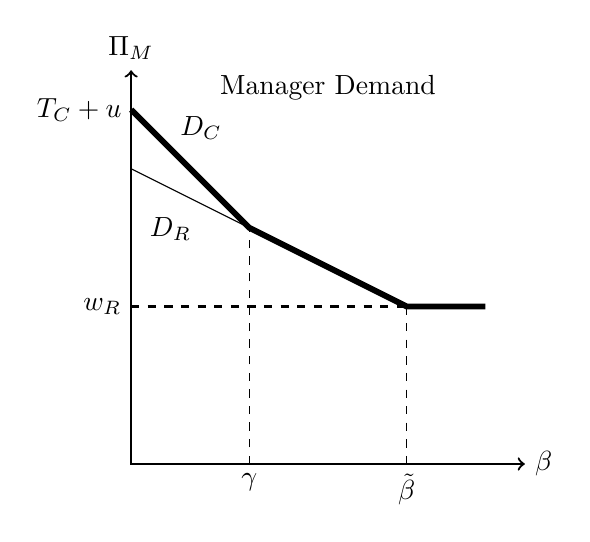
\begin{tikzpicture}[scale=0.5]

\draw[thick,<->] (0,10) node[above]{$\Pi_{M}$}--(0,0)--(10,0) node[right]{$\beta$};

\node [left] at (0,9) {$T_C + u$};
\node [left] at (0,4){ $w_R$};

\node [below] at (7,0) {$\tilde{\beta}$};
\node [below] at (3,0) {$\gamma$};
\node [above right] at (1,8){$D_C$};
\node [above] at (5,9){Manager Demand};

\draw[line width=.75mm](0,9)--(3,6)--(7,4)--(9,4);
\draw (0,7.5)--(3,6);
\node [below] at (1,6.5){$D_R$};

\draw[dashed](7,4)--(7,0);
\draw[dashed](3,0)--(3,6);
\draw[dashed, line width=.5mm](0,4)--(9,4);

\end{tikzpicture}
\end{figure}


\begin{figure}
  \centering
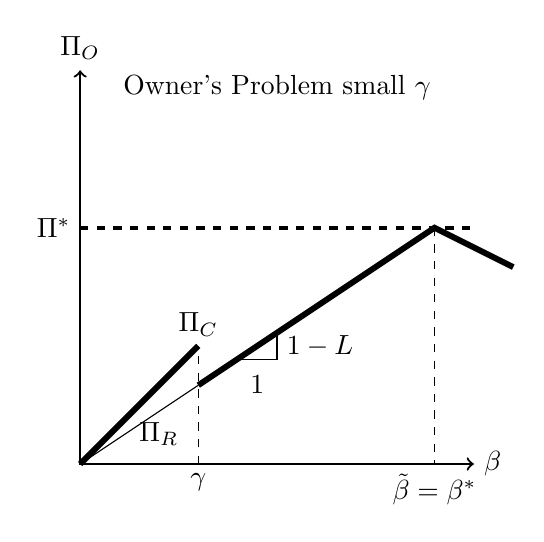
\begin{tikzpicture}[scale=0.5]

\draw[thick,<->] (0,10) node[above]{$\Pi_{O}$}--(0,0)--(10,0) node[right]{$\beta$};

\node [left] at (0,6) {$\Pi^{*}$};

\node [below] at (9,0) {$\tilde{\beta} = \beta^{*}$};
\node [below] at (3,0) {$\gamma$};

% \node [above] at (5,10){};
\node [above] at (5,9){Owner's Problem small $\gamma$};

\draw[line width=.75mm](0,0)--(3,3);
\draw[line width=.75mm](3,2)--(9,6)--(11,5);
\draw (0,0)--(3,2);

\node [above] at (3,3){$\Pi_C$};
\node [below] at (2,1.3){$\Pi_R$};

\draw (4,2.66)--(5,2.66)--(5,3.33);
\node [below] at (4.5,2.5){$1$};
\node [right] at (5,3){$1-L$};

\draw[dashed](9,6)--(9,0);
\draw[dashed](3,0)--(3,3);
\draw[dashed, line width=.5mm](0,6)--(10,6);

\end{tikzpicture}
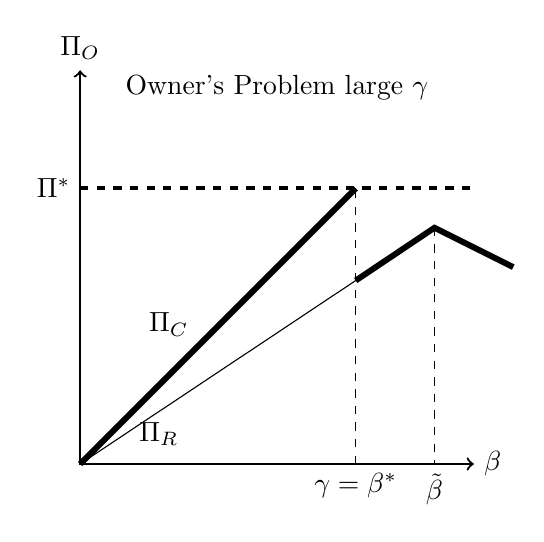
\begin{tikzpicture}[scale=0.5]
  \draw[thick,<->] (0,10) node[above]{$\Pi_{O}$}--(0,0)--(10,0) node[right]{$\beta$};
  \node [left] at (0,7) {$\Pi^{*}$};

\node [below] at (9,0) {$\tilde{\beta}$};
\node [below] at (7,0) {$\gamma = \beta^{*}$};

\node [above] at (5,9){Owner's Problem large $\gamma$};
%\node [above] at (5,10){};

\draw[line width=.75mm](0,0)--(7,7);
\draw[line width=.75mm](7,4.66)--(9,6)--(11,5);
\draw (0,0)--(7,4.66);

\node [above left] at (3,3){$\Pi_C$};
\node [below] at (2,1.3){$\Pi_R$};

\draw[dashed](9,6)--(9,0);
\draw[dashed](7,0)--(7,7);
\draw[dashed, line width=.5mm](0,7)--(10,7);

  
\end{tikzpicture}
\end{figure}

\section{Model}

Consider a world where $T,u$ are observed by all, and during the
hiring process, a potential manager (either relative or contractor)
suggests a function that gives profits as a function of wages. The
Owner observes this, and after seeing the other manager's offer, hires
a worker at a given wage level. Note that the profits given are the
profits that are split between the manager and the owner (after
stealing has occurred.) When there is a tie between the two managers,
this tie is always resolved by the job given to the manager that is
stealing more. The Owner believes that they have spunk and respects
them for it. 

Clearly the owner will accept the one that gives him the higher
payoff.  From this structure we can see that it will not be optimal
for the related manager, who is less productive, to ever steal. As a
contradiction, consider a possible equilibrium where the related
manager is planning to steal (profit is less than $T_R + U$. ), there
is a profitable deviation for the contractor to offer this profit plus
$\epsilon$ more. The contractor will receive the job, although the related
manager could have offered more profit. So he will offer a higher
level of profit than the contractor. This argument will continue in
Bertrand Style until the profit offered is equal to the maximum profit
that the related manager can offer. The more productive manager would
then steal to this level, as the owner cannot do better. The
contractor then receives the job by the tie-breaking rule, and there
is an equilibrium.

When altruism is added to the manager's package the same idea
occurs. Consider first the case where the relative is altruistic, but
still prefers himself. Let $AM$ denote the altruistic manager.

\begin{align*}
  \Pi_{AM} = \alpha \left[ (1-\beta)(1-L) + e(\beta-\gamma) \right] + (1-\alpha)\left[ \beta(1-L-e)
  \right]\\
  \deriv{\Pi_{AM}}{\beta} = (L+e-1)(2\alpha-1) < 0
\end{align*}
where $L+e-1$ is negative since it is $e - (1-L)$ which is the
negative of the reported profit in the contract of related
manager. Note that $2\alpha-1$ is positive as $\alpha \in (\frac{1}{2},1)$.

This means that he still always prefers being paid more money from the
owner, but at less of a degree. There is still no equilibrium where he
steals from the owner, as the owner only values his profits, and the
same Bertrand-Style argument above applies. In any of these
equilibria, the related manager does not receive the job, and thus him
being altruistic does not change the problem at all.

\begin{figure}
  \centering
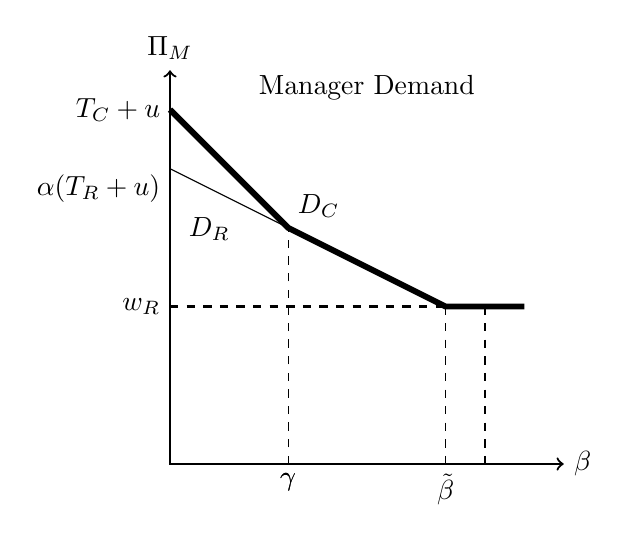
\begin{tikzpicture}[scale=0.5]

\draw[thick,<->] (0,10) node[above]{$\Pi_{M}$}--(0,0)--(10,0) node[right]{$\beta$};

\node [left] at (0,9) {$T_C + u$};
\node [left] at (0,4){ $w_R$};

\node [below] at (7,0) {$\tilde{\beta}$};
\node [below] at (3,0) {$\gamma$};
\node [above right] at (3,6){$D_C$};
\node [above] at (5,9){Manager Demand};

\draw[line width=.75mm](0,9)--(3,6)--(7,4)--(9,4);
\draw (0,7.5)--(3,6);
\node [below] at (1,6.5){$D_R$};

\draw[dashed](7,4)--(7,0);
\draw[dashed](3,0)--(3,6);
\draw[dashed, line width=.5mm](0,4)--(9,4);

\node [left] at (0,7) {$\alpha (T_R + u)$};

\draw[dashed](8,4)--(8,0);
\node [below] at (3,0) {$\gamma$};

\end{tikzpicture}
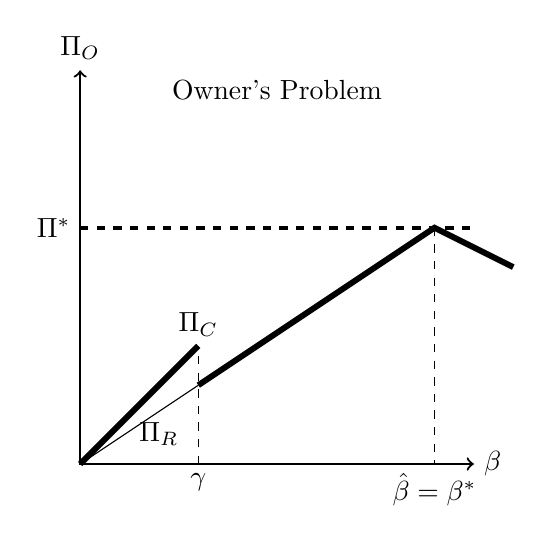
\begin{tikzpicture}[scale=0.5]

\draw[thick,<->] (0,10) node[above]{$\Pi_{O}$}--(0,0)--(10,0) node[right]{$\beta$};

\node [left] at (0,6) {$\Pi^{*}$};

\node [below] at (9,0) {$\hat{\beta} = \beta^{*}$};
\node [below] at (3,0) {$\gamma$};

% \node [above] at (5,10){};
\node [above] at (5,9){Owner's Problem};

\draw[line width=.75mm](0,0)--(3,3);
\draw[line width=.75mm](3,2)--(9,6)--(11,5);
\draw (0,0)--(3,2);

\node [above] at (3,3){$\Pi_C$};
\node [below] at (2,1.3){$\Pi_R$};

\draw[dashed](9,6)--(9,0);
\draw[dashed](3,0)--(3,3);
\draw[dashed, line width=.5mm](0,6)--(10,6);

\end{tikzpicture}
\end{figure}



When the owner is altruistic, the story changes slightly. The owner
now values the well-being of his relative, and values his profit
less. However when considering the contractor's offer, he values only
his profit. The owner will require a higher profit of the contractor
to be indifferent, as long as the relative is making less profit than
he is, and a lower profit when his relative is making more than the
owner. This means that there are equilibria where the son will steal
from his altruistic dad.


When $\beta < \gamma$ neither party wishes to steal. For some values of $\beta$ the
manager will always prefer to hire his son. The utility that is
provided by the son working is positive when $\beta = 0$ and zero for the
contractor. However the slope of the line is smaller than one.

\begin{equation*}
  \deriv{\Pi_{AO}}{\beta} = (1-L)(2\alpha-1) < 1-L < 1
\end{equation*}

It is ambiguous whether or not this line intersects the profit line of
the contractor before $\beta = \gamma$. If it intersects before, then the
manager will hire the contractor after that level of $\beta$. After $\beta =
\gamma$, the contractor will steal down to the utility produced by the
relative manager working, and the relative will not steal by the above
Bertrand Argument. This will continue to the point where the
relative's demand profit equals the reservation wage, occurring at
$\tilde{\beta}$. 

Another case is when the intersection occurs after $\beta = \gamma$. For some
$\beta > \gamma$, the relative provides higher utility than the contractor to
the owner. The relative can then steal down until the owner is at the
utility level of the contractor. The contractor is unable to steal by
the preceding Betrand argument. Let $\eta$ be the intersection between
the utility for the relative, and the profit from the contractor. If
$\tilde{\beta} < \eta$, then the relative will be hired while stealing from
the owner. If $ \tilde{\beta} > \eta$ then the contractor will be hired while
stealing. When they are equal, neither will steal and the owner will
be indifferent between hiring either. 

This means that it does matter whether or not it is the owner or the
son who is altruistic. When the owner is altruistic, he is willing to
hire his relative under certain conditions. However when the relative
is the altruistic one, he is never hired. 

\begin{figure}
  \centering
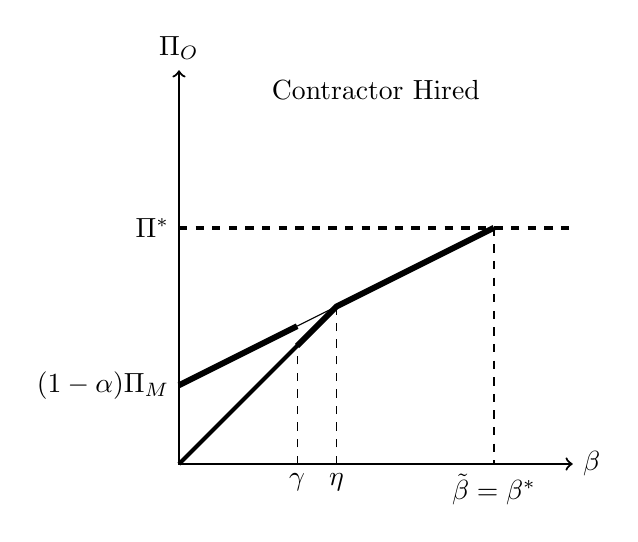
\begin{tikzpicture}[scale=0.5]

\draw[thick,<->] (0,10) node[above]{$\Pi_{O}$}--(0,0)--(10,0) node[right]{$\beta$};

\node [left] at (0,6) {$\Pi^{*}$};

\node [below] at (8,0) {$\tilde{\beta} = \beta^{*}$};
\node [below] at (3,0) {$\gamma$};
\node [below] at (4,0) {$\eta$};
\node [left] at (0,2){ $(1-\alpha) \Pi_M$};

% \node [above] at (5,10){};
\node [above] at (5,9){Contractor Hired};

\draw[line width=.5mm](0,0)--(4,4);
\draw[line width=.75mm](0,2)--(3,3.5);
\draw (3,3.5)--(4,4);
\draw[line width=.75mm](3,3)--(4,4)--(8,6);
%\draw (0,0)--(9,6);

%\node [above] at (3,3){$\Pi_C$};
%\node [below] at (2,1.3){$\Pi_R$};

\draw[dashed](8,6)--(8,0);
\draw[dashed](3,0)--(3,3);
\draw[dashed](4,0)--(4,4);
\draw[dashed, line width=.5mm](0,6)--(10,6);

\end{tikzpicture}
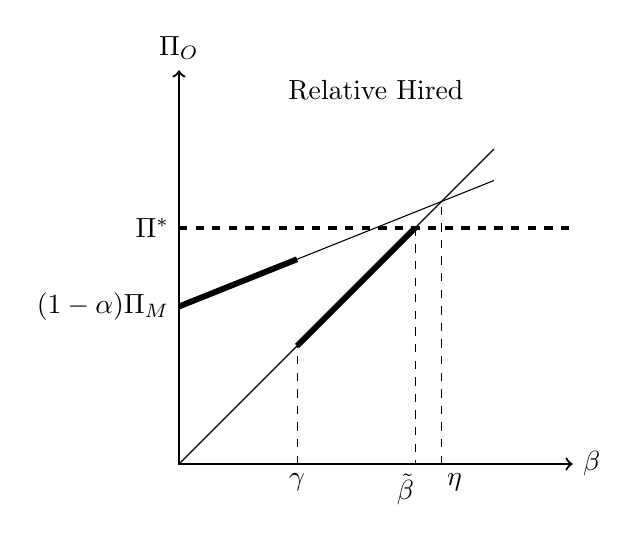
\begin{tikzpicture}[scale=0.5]

\draw[thick,<->] (0,10) node[above]{$\Pi_{O}$}--(0,0)--(10,0) node[right]{$\beta$};

\node [left] at (0,6) {$\Pi^{*}$};

\node [below] at (5.75,0) {$\tilde{\beta}$};
\node [below] at (3,0) {$\gamma$};
\node [below] at (7,0) {$\eta$};
\node [left] at (0,4){ $(1-\alpha) \Pi_M$};

% \node [above] at (5,10){};
\node [above] at (5,9){Relative Hired};

\draw(0,0)--(3,3);
\draw[line width=.75mm](0,4)--(3,5.2);%--(5,6);
\draw (3,5.2)--(5,6)--(8,7.2);
\draw[line width=.75mm](3,3)--(6,6);%--(8,6);
\draw (6,6)--(8,8);

%\node [above] at (3,3){$\Pi_C$};
%\node [below] at (2,1.3){$\Pi_R$};

\draw[dashed](6,6)--(6,0);
\draw[dashed](3,0)--(3,3);
\draw[dashed](6.66,0)--(6.66,6.66);
\draw[dashed, line width=.5mm](0,6)--(10,6);

\end{tikzpicture}
\end{figure}

\section{Is your answer to (b) different if the family is not
  altruistic, but the owner brought up his son to feel guilt, which
  you can interpret as a greater disutility of effort towards
  stealing}

Now, allow for there to be two different values of $\gamma$. The relative
has a higher value of $\gamma$. Note that since the family is not
altruistic, the manager can give the owner higher utility than the
relative can. This prevents the relative from ever stealing, due to
the Betrand argument that has prevented the lower productive member
from stealing before. Therefore increasing the area where the relative
finds it costly to steal has no binding affect on this model. The
relative does not choose to steal, so preventing him from stealing has
no affect on the outcomes.

\section{Under what conditions does the owner prefer to hire his less
  talented son, rather than a more talented unrelated manager?}

The owner prefers to hire his less talented son only when he is
altruistic. When the owner is altruistic, and sufficiently so such
that the intersection between the utility of the owner and the profit
of the contractor occurs after $\tilde{\beta}$, he chooses to hire his
son.  




\end{document}
